\begin {document}

\title {\ZHH \huge 学习ejoy2d——ppm和texture}
\author {\small gaccob}
\date {\small 2004 年 2 月 5 日}
\maketitle

\section* {\ZHH \Large ppm贴图} {
    \begin {itemize}
    \item {pbm, portable bitmap, 单色图(1 bit). }
    \item {pgm, portable gray map, 灰度图. }
    \item {ppm, portable pixel map, 真彩图. }
    \end {itemize}\par

    {pbm / pgm / ppm 图像的文件格式分为两部分: 文件头和数据部分. 一个典型ppm头的sample: }\par
    \begin{lstlisting}[language=bash]
    p6 # `ppm格式`
    1024 1024 # `高, 宽`
    255 # `深度, 不一定就是255`
    \end{lstlisting}

    {ppm的格式有p3和p6, p3表示用ascii码(文本)来表示数据, p6表示以字节码(二进制)来表示, 每一个像素按(r, g, b)的格式来存储. }\par
    \begin{lstlisting}[language=bash]
    P3
    4 4
    15
    0  0  0  0  0  0  0  0  0 15  0 15
    0  0  0  0 15  7  0  0  0  0  0  0
    0  0  0  0  0  0  0 15  7  0  0  0
    15 0 15  0  0  0  0  0  0  0  0  0
    \end{lstlisting}

    {pgm与ppm类似, 格式有p2和p5, p2表示文本, p5表示二进制.}\par
    \begin{lstlisting}[language=bash]
    P2
    18 7
    15
    0 0 0 0 0 0 0 0 0 0 0 0 0  0  0  0  0 0
    0 3 3 3 3 0 0 7 7 7 7 0 0 11 11 11 11 0
    0 3 0 0 0 0 0 7 0 0 0 0 0 11  0  0  0 0
    0 3 3 3 0 0 0 7 7 7 0 0 0 11 11 11  0 0
    0 3 0 0 0 0 0 7 0 0 0 0 0 11  0  0  0 0
    0 3 0 0 0 0 0 7 7 7 7 0 0 11 11 11 11 0
    0 0 0 0 0 0 0 0 0 0 0 0 0  0  0  0  0 0
    \end{lstlisting}

    {对于pbm来说, 格式为p1, 但是文件头中没有最大颜色, 因为用0和1来表示就可以了.}\par
    \begin{lstlisting}[language=bash]
    P1
    24 7
    0 0 0 0 0 0 0 0 0 0 0 0 0 0 0 0 0 0 0 0 0 0 0 0
    0 1 1 1 1 0 0 1 1 1 1 0 0 1 1 1 1 0 0 1 1 1 1 0
    0 1 0 0 0 0 0 1 0 0 0 0 0 1 0 0 0 0 0 1 0 0 1 0
    0 1 1 1 0 0 0 1 1 1 0 0 0 1 1 1 0 0 0 1 1 1 1 0
    0 1 0 0 0 0 0 1 0 0 0 0 0 1 0 0 0 0 0 1 0 0 0 0
    0 1 0 0 0 0 0 1 1 1 1 0 0 1 1 1 1 0 0 1 0 0 0 0
    0 0 0 0 0 0 0 0 0 0 0 0 0 0 0 0 0 0 0 0 0 0 0 0
    \end{lstlisting}

    \par{参考文章: \href{http://www.cppblog.com/windcsn/archive/2005/11/11/ppm.html}{http://www.cppblog.com/windcsn/archive/2005/11/11/ppm.html}}
}

\section*{\ZHH \Large ejoy2d中的ppm源码}{
    {ejoy2d中的ppm贴图的处理都在lib/ppm.h和lib/ppm.c中. ejoy2d中用pgm贴图来描述alpha通道, 用ppm贴图来描述rgb通道. }\par
    \begin{lstlisting}[language=C]
struct ppm {
    // `指ppm贴图的格式, p1-p6分别对应1-6`
    int type;
    // `图像的深度, 一般有255(8位)和15(4位)`
    int depth;
    // `步长, alpha是1, rgb是3, rgba就是4`
    int step;
    // `长 \& 宽`
    int width;
    int height;
    // `图像数据`
    uint8_t *buffer;
};

// `载入ppm文件头`
static int
ppm_header(FILE *f, struct ppm *ppm) {
    ......
    // `格式`
    char c = 0;
    sscanf(line, "P%c", &c);
    ......
    // `长 \& 宽`
    sscanf(line, "%d %d", &(ppm->width), &(ppm->height));
    ......
    // `图像深度, 这里就是255或者15`
    sscanf(line, "%d", &(ppm->depth));
    .......
}

// `载入ppm文件数据`
// `这里会根据type(p1, p2, ...)的不同, 做对应的解析并载入`
// `skip是为了有一个初始offset(适用于rgb ppm载入alpha的情况)`
static int
ppm_data(struct ppm *ppm, FILE *f, int id, int skip) {
    ......
    switch(id) {
        case '3':    // RGB text
            ......
        case '2':    // ALPHA text
            ......
        case '6':    // RGB binary
            .......
        case '5':    // ALPHA binary
            ......
    }
}

// `载入ppm文件, 调用ppm\_header()和ppm\_data()完成.`
// `如果是rgba, 需要从两个贴图文件一起载入(会做一致性校验)`
static int
loadppm_from_file(FILE *rgb, FILE *alpha, struct ppm *ppm) {
    ......
}

// `载入ppm文件的lua接口`
// `lua输入参数:`
// `     string ppm\_name`
// `输出lua结果:`
// `     string format(这里约定的格式有: RGBA8, RGB8, ALPHA8, RGBA4, RGB4, ALPHA4)`
// `     int width`
// `     int height`
// `     table buffer(ppm数据部分)`
static int
loadppm(lua_State *L) {
    ......
}

// `载入ppm文件到texture(纹理)的lua接口`
// `lua输入参数:`
// `     string ppm\_name`
static int
loadtexture(lua_State *L) {
    // `载入ppm文件, 调用loadppm\_from\_file()完成`
    ......

    // `根据ppm的格式, 设置texture的格式`
    int type = 0;
    if (ppm.depth == 255) {
        if (ppm.step == 4) {
            type = Texture2DPixelFormat_RGBA8888;
        } else if (ppm.step == 3) {
            type = Texture2DPixelFormat_RGB888;
        } else {
            type = Texture2DPixelFormat_A8;
        }
    }
    // `depth为15, 需要根据step的不同(即texture格式的不同)做buffer的转换`
    else {
        if (ppm.step == 4) {
            ......
        } else if (ppm.step == 3) {
            ......
        } else {
            ......
        }
    }

    // `最后加载texture, 这一块具体可以参照下节`
    const char * err = texture_load(id, type, ppm.width, ppm.height, ppm.buffer);
    free(ppm.buffer);
    if (err) {
        return luaL_error(L, "%s", err);
    }
    return 0;
}

// `根据format(上面描述的RGBA8等格式), 设置ppm数据: type, depth, step`
static void
ppm_type(lua_State *L, const char * format, struct ppm *ppm) {
    ......
}

// `从lua中读取数据, 保存rgb的ppm贴图(写文件), P6二进制格式.`
static void
save_rgb(lua_State *L, int step, int depth) {
    ......
}

// `从lua中读取数据, 保存alpha的pgm贴图(写文件), P5二进制格式.`
static void
save_alpha(lua_State *L, int step, int depth, int offset) {
    ......
}

// `保存ppm文件的lua接口, 调用save\_rgb()和save\_alpha()实现, 写文件.`
// `lua输入参数:`
// `     string save\_filename(保存的文件名)`
// `     string format(同上)`
// `     int width`
// `     int height`
// `     table buffer(ppm数据部分)`
static int
saveppm(lua_State *L) {
    ......
}

// `lua的导出接口`
int
ejoy2d_ppm(lua_State *L) {
    luaL_Reg l[] = {
        { "texture", loadtexture },
        { "load", loadppm },
        { "save", saveppm },
        { NULL, NULL },
    };
    luaL_newlib(L,l);
    return 1;
}

    \end{lstlisting}
}

\section*{\ZHH \Large texture纹理}{
    {这部分内容大部分来自\href{http://www.cnblogs.com/shengdoushi/archive/2011/01/13/1934181.html}{http://www.cnblogs.com/shengdoushi/archive/2011/01/13/1934181.html}}\par
    {纹理实际上是一个二维数组, 其元素是一些颜色值, 每一元素称之为纹理像素(texel). OpenGL以一个整形id来作为句柄管理纹理对象. 通常, 一个纹理映射的步骤是:}
    \begin{enumerate}
    \item{创建纹理对象, 获得一个句柄id.}
    \item{设定过滤, 定义了OpenGL显示图像的效果. }
    \item{加载纹理数据, 将图像数据赋值给纹理对象. }
    \item{绑定纹理对象. }
    \item{纹理映射, 将绑定纹理的数据绘制到屏幕. }
    \end{enumerate}
    \par

    {纹理有自己的一套坐标系(Figure \ref{label_texture_corrd}). }
    \begin{figure}[htbp]
        \centering
        \caption{\label{label_texture_corrd} 纹理坐标系}
        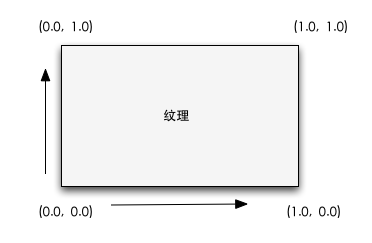
\includegraphics[width=280pt, keepaspectratio]{texture_coord.png}
    \end{figure}
    \par

    {纹理映射: 是指将纹理绘制到屏幕的过程, 这中间会有坐标系的转换(Figure \ref{label_texture_mapping}). }
    \begin{figure}[htbp]
        \centering
        \caption{\label{label_texture_mapping} 纹理映射}
        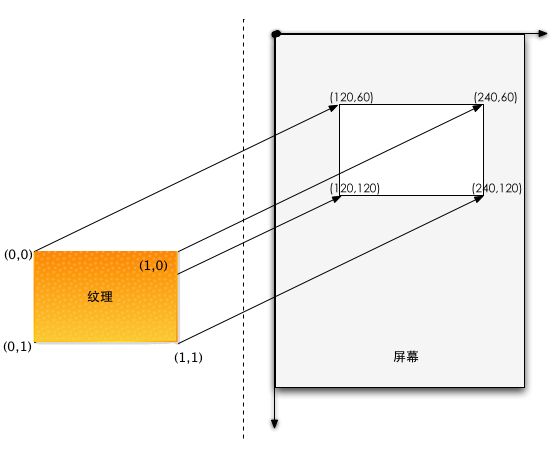
\includegraphics[width=400pt, keepaspectratio]{texture_mapping.png}
    \end{figure}
    \par
}

\section* {\ZHH \Large ejoy2d中的texture源码}{
    {ejoy2d中关于texture的代码大部分都在lib/texture.h和lib/texture.c中. }\par
    \begin{lstlisting}[language=C]
// `这是ejoy2d支持的纹理格式`
#define Texture2DPixelFormat_RGBA8888 1
#define Texture2DPixelFormat_RGBA4444 2
#define Texture2DPixelFormat_PVRTC4 3
#define Texture2DPixelFormat_PVRTC2 4
#define    Texture2DPixelFormat_RGB888 5
#define Texture2DPixelFormat_RGB565 6
#define Texture2DPixelFormat_A8 7

// `这是texture对象, 这里的id就是OpenGL的句柄, invw和invh避免了做除法`
struct texture {
    int width;
    int height;
    float invw;
    float invh;
    GLuint id;
};

// `内存池来管理纹理对象, 默认最大128对象`
struct texture_pool {
    int count;
    struct texture tex[MAX_TEXTURE];
};
static struct texture_pool POOL;

// `从数据(一般是贴图)加载纹理`
const char *
texture_load(int id, int pixel_format, int pixel_width, int pixel_height, void *data) {
    ......

    // `OpenGL创建texture`
    glGenTextures(1, &tex->id);

    // `指定当前的纹理单元`
    glActiveTexture(GL_TEXTURE0);

    // `这里shader会调用glBindTexture()绑定纹理`
    shader_texture(tex->id);

    // `缩小|放大过滤器, 线性滤波`
    glTexParameteri( GL_TEXTURE_2D, GL_TEXTURE_MIN_FILTER, GL_LINEAR );
    glTexParameteri( GL_TEXTURE_2D, GL_TEXTURE_MAG_FILTER, GL_LINEAR );
    // `GL\_CLAMP\_TO\_EDGE使得超出边缘的部分与边缘保持一致, 有个学名叫"箝位"`
    glTexParameteri( GL_TEXTURE_2D, GL_TEXTURE_WRAP_S, GL_CLAMP_TO_EDGE );
    glTexParameteri( GL_TEXTURE_2D, GL_TEXTURE_WRAP_T, GL_CLAMP_TO_EDGE );

    // `根据纹理格式来分别加载数据`
    switch(pixel_format) {
         ......
    }
    return NULL;
}

// `卸载(删除)纹理对象`
void
texture_unload(int id) {
    if (id < 0 || id >= POOL.count)
        return;
    struct texture *tex = &POOL.tex[id];
    if (tex->id == 0)
        return;
    // `从OpenGL中删除纹理对象`
    glDeleteTextures(1,&tex->id);
    tex->id = 0;
}

// `纹理的坐标系转换`
void
texture_coord(int id, float *x, float *y) {
    if (id < 0 || id >= POOL.count) {
        *x = *y = 0;
        return;
    }
    struct texture *tex = &POOL.tex[id];
    // `相当于 x/texture\_x, y/texture\_y, 这里的用法后面看sprite的时候再看`
    *x *= tex->invw;
    *y *= tex->invh;
}
    \end{lstlisting}
}

\end {document}
